\documentclass[a4paper,
               %boxit,
               %titlepage,   % separate title page
               %refpage      % separate references
              ]{jacow}
%
% CHANGE SEQUENCE OF GRAPHICS EXTENSION TO BE EMBEDDED
% ----------------------------------------------------
% test for XeTeX where the sequence is by default eps-> pdf, jpg, png, pdf, ...
%    and the JACoW template provides JACpic2v3.eps and JACpic2v3.jpg which
%    might generates errors, therefore PNG and JPG first
%
\makeatletter%
	\ifboolexpr{bool{xetex}}
	 {\renewcommand{\Gin@extensions}{.pdf,%
	                    .png,.jpg,.bmp,.pict,.tif,.psd,.mac,.sga,.tga,.gif,%
	                    .eps,.ps,%
	                    }}{}
\makeatother

% CHECK FOR XeTeX/LuaTeX BEFORE DEFINING AN INPUT ENCODING
% --------------------------------------------------------
%   utf8  is default for XeTeX/LuaTeX 
%   utf8  in LaTeX only realises a small portion of codes
%
\ifboolexpr{bool{xetex} or bool{luatex}} % test for XeTeX/LuaTeX
 {}                                      % input encoding is utf8 by default
 {\usepackage[utf8]{inputenc}}           % switch to utf8

\usepackage[USenglish]{babel}			 

\usepackage[final]{pdfpages}
\usepackage{multirow}
\usepackage{ragged2e}


\usepackage{amsmath}
\usepackage{breqn}

\usepackage[]{algorithm2e}
\SetKwComment{Comment}{$\triangleright$\ }{}

\usepackage{svg}

%\usepackage{draftwatermark}
%\SetWatermarkText{Draft 2017-07-02}
%\SetWatermarkScale{0.7}
%\SetWatermarkLightness{0.9}

\usepackage{hyperref}
\PassOptionsToPackage{hyphens}{url}\usepackage{hyperref}

  
%
% if BibLaTeX is used
%
\ifboolexpr{bool{jacowbiblatex}}%
 {%
  \addbibresource{jacow-test.bib}
  \addbibresource{biblatex-examples.bib}
 }{}
\listfiles

%
% command for typesetting a \section like word
%
\newcommand\SEC[1]{\textbf{\uppercase{#1}}}

%%
%%   Lengths for the spaces in the title
%%   \setlength\titleblockstartskip{..}  %before title, default 3pt
%%   \setlength\titleblockmiddleskip{..} %between title + author, default 1em
%%   \setlength\titleblockendskip{..}    %afterauthor, default 1em

%\copyrightspace %default 1cm. arbitrary size with e.g. \copyrightspace[2cm]

% testing to fill the copyright space
%\usepackage{eso-pic}
%\AddToShipoutPictureFG*{\AtTextLowerLeft{\textcolor{red}{COPYRIGHTSPACE}}}

\begin{document}

\title{ PLC Factory: Automating routine tasks in large-scale PLC software development}

\author{G. Ulm\thanks{gregor.ulm@alumni.lse.ac.uk}\textsuperscript{1}, F. Bellorini, D. Brodrick, R. Fernandes, N. Levchenko, D. Piso Fernandez,\\ European Spallation Source ERIC, Lund, Sweden\\
		\textsuperscript{1}also at Chalmers University of Technology, Gothenburg, Sweden
		}
	
\maketitle

% TODO
% . check style of references
% . add title of Ricardo's forthcoming paper on CCDB


\begin{abstract}
At the European Spallation Source ERIC (ESS) in Lund, Sweden, the entire facility including all its instruments will be controlled by a large number of programmable logic controllers (PLCs). Programming PLCs, however, entails a significant amount of repetition. It is thus an error-prone and time-consuming task. Given that PLCs interface with hardware, this involves economic aspects as well, due to the fact that programming errors may cause damage to equipment. With PLC Factory, we managed to automate repetitive tasks associated with PLC programming and interfacing PLCs from EPICS. This tool is used in production at ESS and has led to a large increase in productivity compared to the previous status quo. We describe PLC Factory as well as its embedded domain-specific programming language PLCF$^\sharp$, which it is built upon.
\end{abstract}



\section{Introduction}
The European Spallation Source ERIC~(ESS) in Lund is building large-scale infrastructure that is projected to include hundreds of programmable logic controllers (PLCs). Of particular concern is that PLCs directly control hardware, thus erroneous instructions may lead to damage to equipment. An additional problem is that programming PLCs is a rather repetitive affair. With a small number of PLCs, the tedium is certainly manageable. However, given the future large-scale deployment of PLCs at ESS, we were motivated to look into ways of automating some of the tedium associated with PLC programming with the dual goal of both saving time and increasing reliability as computers are better suited to repetitive tasks than humans.

The structure of this paper is as follows: After describing the problem we were facing at ESS in some detail, we present a high-level description of our solution, i.e.\ the application PLC Factory. That section covers how dependencies between devices are implicitly modeled by an in-house database, the role of template files and how they are processed, the detailed execution of PLC Factory via pseudocode, a description of the substitutions that are performed by a custom domain-specific language, a brief discussion of how we check for consistency in the data we produce, and an analysis of the computational cost of PLC Factory. This is followed by a short section on related work, and a section on future work.



\section{Problem Description}
ESS uses a database for configuration management, the Controls Configuration Database (CCDB). It is conceptually similar to a system at CERN with the very same name~\cite{CCDB-CERN}. Yet, CCDB at ESS was developed from scratch. The Facility for Rare Isotope Beams (FRIB) at Michigan State University is another user of CCDB. CCDB contains static device information of the entire instrumentation hardware at ESS. %Details are described by Fernandes~\cite{CCDB-ESS} .

The problem we wanted to solve was to automatically generate both EPICS database records as well as code blocks in Structured Control Language~(SCL) for the Siemens product TIA Portal. The former were intended to be complete records so that they could easily be imported into our local EPICS installation, the ESS EPICS Environment~(EEE). The Experimental Physics and Industrial Control System~(EPICS) is a distributed control system for scientific instruments \cite{EPICS}. The goal with regards to SCL code generation was to produce code blocks with relevant device information for a particular PLC. Furthermore, we wanted to explore approaches that allow the dynamic computation of values, such as memory addresses, which, for instance, may increase in fixed intervals.

CCDB stores information for each device instance and device type. Devices can be in two kinds of relations. First, a device is in a \emph{controls} relationship with each device it controls. This is a finite number of controlled devices, which may be zero. Second, a device may also be in a \emph{controlled-by} relationship that states which devices it is controlled by. In order to refer to these hierarchies of dependencies, we will use the term \emph{dependency tree} in the following, or simply just \emph{tree}. Those trees are only implicitly described by CCDB entries.

Before the advent of PLC Factory, a PLC programmer would use a number of templates according to device type, populate them \emph{manually} with values taken from CCDB, hope to not have made a mistake, and use the resulting files for configuring EEE or as a starting point for continuing PLC programming in TIA Portal. This approach is repetitive, error-prone, and does not scale well with increasingly larger dependency trees. Thus, we were looking for a solution that handles the following cases of substitutions in template files:

\begin{enumerate}

\item direct substitution, i.e.\ for a given device~$d$, use property~$p$ as specified in the corresponding CCDB entry for $d$

\item enabling shared properties between devices, in order to remove redundancies in CCDB

\item automatically managing counters to specify PLC memory address offsets in EPICS database records

\end{enumerate}

The first problem is straightforward as it is based on a simple database lookup. The motivation behind the second issue is that it is not uncommon that devices share property names and values. This was originally reflected by duplication of data in CCDB. However, we wanted to reduce such redundancies in order to decrease the maintenance burden. The third problem is a greater challenge as part of creating the output file requires manually incrementing memory addresses. It also promised a much bigger payoff, considering that this task, when creating records for many devices, easily involves hundreds of modifications. While not inherently difficult, adjusting memory addresses manually is nonetheless a error-prone and time-consuming task. 



\section{Solution}
PLC Factory is an application written in Python 2.7 that automates the three kinds of substitutions we just outlined.\footnote{PLC Factory is an open-source product, licensed under the third version of the GNU General Public License (GNU GPLv3). The source code  is available at the following repository: \texttt{https://bitbucket.org/\linebreak europeanspallationsource/ics_plc_factory}.} Those automatic substitutions remove most if not all of the repetition we encounter when engaging in large-scale PLC software development. Starting with the foundational concept of a \emph{dependency tree}, we are going to describe the steps PLC Factory performs in successively greater detail. After presenting a high-level overview, we will move on to pseudocode and eventually dissect PLCF$^\sharp$, the embedded domain specific language that is at the core of PLC Factory, and which enables the expressivity and flexibility we are about to discuss.

\subsection{Dependency Trees}
Since CCDB describes dependency relationships between devices, this information can be used to construct a \emph{dependency tree} that explicitly models those relationships. Let us present a simple example: Consider an element $r$, which is the starting point for PLC Factory and the root of the tree we intend to construct. The root device $r$ controls the devices $u_1$ and $u_2$, of which the former controls $v_{11}$ and $v_{12}$, and the latter $v_{21}$. This is illustrated in Fig.\ \ref{fig:deviceTree}. In a production setting such a tree can be arbitrarily deep. Every unique device is of a particular device type, for instance a PLC or a vacuum pump. A dependency tree may contain several devices that are of the same device type.

\begin{figure}[h]
\centering
  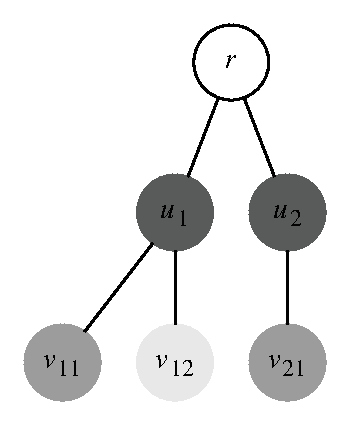
\includegraphics[scale=0.8]{figures/deviceTreeCropped.eps}
  \caption{Example of a dependency tree. Different shadings indicate different device types.}
  \label{fig:deviceTree}
\end{figure}

% create a GraphViz image file with correctly rendered subscripts on OSX:
% dot -Tpdf:cairo -v deviceTree.dot -o deviceTree.pdf



\subsection{Template files}
PLC Factory takes a list of template IDs as one of its inputs. One such ID may be \texttt{EPICS} or \texttt{TIA}, where the former may designate templates that are used for creating an EPICS database records file, and the latter SCL code blocks for TIA Portal. A device type may have template files with particular IDs attached to it in CCDB. In general, template files are text files with a fixed structure. Through processing via PLC Factory, certain fields within a template file are replaced. A simplified example is the substitution of a field \texttt{DEVICE\_NAME} in a template by the concrete name of a device that is an instance of the device type this template is associated with.

In addition, \emph{header} and \emph{footer} files with a template ID can be attached to a device type. Those files may be static, but they could also be regular template files. The main reason why headers and footers constitute a separate category is that the header needs to be prepended to the resulting output file, and the footer appended. For other templates, the ordering could be arbitrary, which implies that even though the output of PLC Factory is deterministic, i.e.\ given identical inputs, two runs will result in identical output, there are many possible valid outputs for a given input.

\subsection{Processing template files}
Assume that, in Fig.\ \ref{fig:deviceTree}, the root device $r$ is of device type $d_0$, devices $u_i$ are of device type $d_1$, $v_{11}$ and $v_{21}$ are of device type $d_2$, while $v_{12}$ is of a different type, $d_3$. We define the operator $\oplus$ as a shorthand for processing template files. This operator is applied to a device instance $x$ and a specific template. Templates are retrieved by a function $t$ that takes as its input a template ID like \texttt{EPICS} and the device type of $x$, which is determined by the function $d$ applied to device $x$. Thus, the resulting operation is $x \oplus t(\mathit{id}, d(x))$. If there is no such template attached to CCDB, then no output for that particular device within this tree is produced. Conceptually, PLC Factory skips such nodes in the tree.

In addition, we define the header file $h(\mathit{id}, d(r))$ as well as the footer file $f(\mathit{id}, d(r))$. The root $r$ has no other templates associated with it. The concatenation operator is given by the $+$ symbol. Template processing has a higher precedence than concatenation. PLC Factory processes a tree level by level. The resulting order of the output resulting from processing the tree in Fig.\ \ref{fig:deviceTree} is a concatenation of the following form:

\begin{multline}
      r          \oplus h(\mathit{id}, d(r))
+ \  u_1     \oplus t(\mathit{id}, d(u_1))       +  \dots  \\
+ \  v_{11} \oplus t(\mathit{id}, d(v_{11}))   +  \dots + \ r  \oplus f(\mathit{id}, d(r))      
\end{multline}

This example describes PLC Factory on a high-level, but glosses over some of the more intricate steps in template processing, such as user-specified computations, or resolving references to properties of both the current device as well as to devices on a higher level in the hierarchy. These features are discussed in the subsection on PLCF$^\sharp$ further below.

\subsection{Detailed Execution Order}
PLC Factory takes a root device $r$ as well as a list $\mathit{ids}$ of template IDs as arguments. As stated in the previous subsection, template IDs specify the kind of the desired output file, for instance \texttt{EPICS} for EPICS database records of a tree. For each template ID $id$, the following algorithm is executed. 

\begin{algorithm}
 \label{alg:algo}
 \KwData{CCDB, root device $r$, template ID $id$}
 \KwResult{list \emph{out} containing text for post-processing}
\Begin{
 $\mathit{out} \leftarrow  \varnothing$  \Comment*[f]{collected output}  \\
 $\mathit{ds} \leftarrow r$   \Comment*[f]{list of devices} \\
 \While{ ds \emph{not $\varnothing$ } }{
  $d \leftarrow$  $ds$.pop() \\
  $cs \leftarrow $ $d$.controls()  \Comment*[f]{CCDB lookup}  \\
  \While{ cs \emph{not} $\varnothing$  }{
    $c \leftarrow$ $\mathit{cs}$.pop() \\
    \If{  $ t(\mathit{id}, d(c)) \in $ CCDB} { 
           $\mathit{out} \leftarrow \mathit{out} + c \oplus  t(\mathit{id}, d(c))  $  \\
           $\mathit{cs}' \leftarrow c.$controls() \\
           $\mathit{ds} \leftarrow \mathit{ds} + \mathit{cs}'$ \\
   }
  }  
 }
$\mathit{out} \leftarrow r \oplus  h(\mathit{id}, d(r))    + \mathit{out} + r \oplus f(\mathit{id}, d(r))   $   \\
 }
 \caption{Processing a dependency tree}
\end{algorithm}

The method \texttt{controls()} queries CCDB in order to determine which devices $\mathit{cs}$ are controlled by a given device $d$, while the method \texttt{pop()} removes the first element from a list, and returns it. The function $t$ retrieves templates, while the function $d$ determines the type of a device, as described further above.

All lookup operations are memoised, i.e.\ their results are stored in-memory, in a hash table. Whenever a lookup is performed, this hash table is first queried. Only if a certain device has not yet been encountered, a request is sent to CCDB via the network. This means that PLC Factory will not issue unnecessary requests to CCDB as in-memory data is always queried first. This fact is particularly relevant for the later subsection on scaling behavior of PLC Factory. % on page \pageref{subsec:runtime}.

PLC Factory creates output files by processing a dependency tree in a consistent order. In general, templates are attached to device types, but CCDB also contains information related to each device instance. For a given template ID, template processing of a device $d$ involves retrieving both the template associated with the device type of $d$ as well as retrieving the instance-specific properties of $d$ from CCDB. Furthermore, the root element of a tree may have a header or footer file attached to it, which are processed at the very end.

\subsection{\emph{PLCF$^\sharp$}, an embedded domain-specific language}
\label{subsec:plcf}
A central feature of PLC Factory is the embedded domain-specific programming language PLCF$^\sharp$. Essentially, PLCF$^\sharp$ is a mini programming language for simple expressions, which are embedded in template files. For each such expression, PLCF$^\sharp$ performs a number of substitutions and evaluations, with the goal of eventually producing a valid Python expression. Those Python expressions are finally evaluated and their resulting values placed in a template file with the goal of producing the final output. PLC developers define PLCF$^\sharp$ expressions within template files. Those expressions are evaluated while PLC Factory processes the set of template files that are associated with a tree.

PLCF$^\sharp$ solves the following two problems:

\subsubsection{Shared property values}
CCDB contains properties of each device. However, it is a relatively frequent occurrence that a device $d'$ which is controlled by $d$ shares some of its properties as well as the values associated with them. We refer to this as \emph{shared property values}. A straightforward solution is to store those property values in CCDB for both $d$ and $d'$. However, this leads not only to redundancies, it also increases the maintenance burden as property values need to be updated for several devices at once. Due to its repetitiveness, this is a potentially error-prone activity.

\subsubsection{Memory address management}
A potentially even more tedious and repetitive task is the manual management of memory addresses, and their stepwise increments in EPICS records and SCL files. In an SCL source code file for a moderately complex tree, a PLC developer may need to enter many hundreds of memory locations, and keep different step sizes in mind. \\

The general principle is that a PLC developer has the freedom to define an unlimited number of expressions in PLCF$^\sharp$ as part of a template file. Their general format is $[\mathit{PLCF^\sharp} <\mathit{expression}>]$. PLCF$^\sharp$ expressions are eventually transformed into valid Python expressions. PLCF$^\sharp$ knows a  restricted number of keywords. With the exception of counter variables and \texttt{\#HASH}, these keywords are not discussed in this paper, however. Furthermore, it is possible to call user-defined functions, which need to be defined in an external source code file. This is an advanced feature, which we will not discuss it in this paper either.



\subsubsection{Resolving local device properties}
This is the first of three increasingly complex use cases that illustrate the power and flexibility of PLCF$^\sharp$. A user may want to perform simple arithmetic operations involving properties related to the current device, e.g.\ \\

\texttt{[PLCF\# DataBlockStartOffset + 1]} \\

This means that the value of the CCDB property \texttt{DataBlockStartOffset} associated with the current device will be used for this computation. The lookup happens in reverse, though. Instead of looking up a property name that is part of a PLCF$^\sharp$ expression in CCDB, PLC Factory requests all property names and values for the device it is currently processing. Afterwards, PLC Factory looks for each property name in the provided PLCF$^\sharp$ expression. If there is a match, it performs a substitution with the associated property value from CCDB.

While this approach may appear counter-intuitive at first, it ensures that PLC Factory is highly flexible as it does not need to have any knowledge of concrete property names. In contrast, a more straightforward substitution would be based on known property names, similar to how certain keywords, e.g.\ \texttt{\#HASH}, are handled. Such an approach, however, would be much more difficult to maintain. In contrast, with the chosen approach a user can define any property name in CCDB and rest assured that its value will be correctly used when processing template files --- as long as both the property name in CCDB and the property name in the associated template file match. This does not require any modification of PLC Factory itself as the tool is fully agnostic of property names.

%    Implementation detail:    
%
%    Sorting property names from longest to shortest avoids
%    the potential issue that a PLCF# expression can't be fully
%    evaluated when a property name is part of another property name of
%    the same device.
%    
%    In more technical terms: the list of propery names that are
%    retrieved via the method keys() is neither sorted nor deterministic,
%    i.e. multiple calls may result in different permutations of the
%    same elements.
%    
%    In PLC Factory, property names are processed one by one, as they 
%    are encountered (see the for-loop below). Further, there is no
%    semantic analysis of PLCF# expressions. Thus, without
%    sorting, it may happen that a property name "foo" is processed before
%    a property name "foobar", but processing the former would leave "bar"
%    in the resulting expression. This would be bad enough, but imagine
%    what would happen if there was a property name "bar" left to process!
%    
%    With sorting by property names by length in reverse, i.e. from longest
%    to shortest, "foobar" is processed before "foo", so the issue described
%    above is entirely avoided. For the curious, this approach is similar
%    to the "maximal munch" concept in compiler theory.

\subsubsection{Resolving shared device properties}
Recall that properties may be shared by devices within a tree. PLCF$^\sharp$ knows the special operator $\uparrow$, pronounced as "up" and represented by the caret symbol (\texttt{\textasciicircum}).\footnote{As we later learnt, this design decision happened to be an unintentional throwback to the early days of computing. The original 1963 ASCII standard knew an upwards arrow symbol. However, it was replaced by a caret in its 1965 revision.} Using the \emph{up} operator, a PLC developer only needs to update a shared property for a parent device in the tree.\footnote{This is a simplification. In reality, the root of a dependency tree does not need to contain the property value a dependent device is using. Instead, PLC Factory will traverse the \emph{entire} implicit tree that is specified by CCDB. Thus, a shared property may eventually be looked up in a device that is located many levels above the root of the chosen dependency tree.} All child nodes can subsequently refer to this one property. In code, it looks as follows: \\

\texttt{[PLCF\# \textasciicircum(DataBlockStartOffset) + 1]} \\

Being able to refer to shared properties in this way greatly reduces the maintenance burden as we only need to update, in the case of a property that is universally shared among devices within a tree, one single entry in CCDB instead of a potentially very large number of entries.


\subsubsection{Handling global counter variables}
Template files may contain global counter variables. In order to make PLCF$^\sharp$ properly handle those variables, the only requirement is to specify the increment of the used counters in a template file. Modifying the previous example, one of our template files may contain the following statement:\\

\texttt{[PLCF\# \textasciicircum(DataBlockStartOffset) + Counter1]} \\

Processing counter variables happens as a separate post-processing step. To refer to the algorithm presented earlier, post-processing is performed on the output \emph{out}, and subsequently written to a text file. Counter variables dynamically change as they may be incremented with each additionally processed template. While part of the motivation behind automating memory allocations and computing offsets is due to wanting to fill up the available memory block by block in a consistent manner, the main reason for automating this task emerges in the interplay between EPICS database records and their corresponding SCL files. This is briefly discussed in the subsection on consistency checks further below.


\subsection{Evaluation order}

The evaluation order of a PLCF$^\sharp$ expression is as follows:

\begin{enumerate}
\item look up shared properties
\item look up local properties
\item process counter variables
\item evaluate the resulting expression in Python
\end{enumerate}

This order is always maintained, although each of the first three steps is optional. After the last step, the PLCF$^\sharp$ designators, i.e. \texttt{[PLCF\#} and the closing square bracket \texttt{]} are dropped and the computed value is inserted into the output.

\subsection{Consistency checks}
One of the goals of PLC Factory is to make large-scale PLC programming less error-prone. Thus, we implemented a measure for indicating whether properties and property values associated with the devices within a tree have been modified, possibly by a different user. This is, for instance, useful in order to quickly verify whether there have been changes of related data in CCDB after creating a set of output files. Assume a user receives SCL and EPICS files for a given dependency tree. By comparing the hash value contained in the header of both the SCL source file and the EPICS database records, it can be quickly verified whether both files refer to the exact same tree. The hash value is used to compare the consistency between structurally different files. Thus, using a tool like \texttt{diff} would not be feasible. Time stamps would not be feasible either, as those would differ between two executions of PLC Factory even if all values of the dependency tree were the same.

It is important that the memory locations in a set of EPICS database records correspond to the associated SCL file. The reason is that a mismatch may lead to unexpected behavior, like opening the wrong valve. In order to avoid that kind of problem, it is essential to quickly verify the consistency of both SCL files and EPICS database records. PLC Factory computes a hash value for a tree in a deterministic manner. A user is able to access this value by placing the keyword \texttt{\#HASH} in a template file. This value is also printed to the command line after processing a dependency tree with PLC Factory.


\subsection{Scaling behavior}
\label{subsec:runtime}
PLC Factory is a highly efficient tool that scales very well in practice. The bottleneck of the execution is due to input/output operations like accessing CCDB via the network, downloading template files, opening those files, and writing the final output. For every device type and every device in a tree only one CCDB query is performed. Accessing information repeatedly queries an in-memory cache instead. As a consequence, PLC Factory runs in linear time, viz.\ $O(m + n) = O(n)$, where $m$ is the number of device types, of which there is one template associated with each device type, and $n$ the number of devices.\footnote{In case the result of $O(n)$ is not immediately obvious: a tree contains $n$ unique devices which are instances of $m$ device types. We also know that the number of device types is at most as large as the number of unique devices. In reality, though, $m$ is much less than $n$. Thus, we can identify a leading coefficient, which is subsequently dropped: $O(m + n) \le O(2n) = O(n)$.} CCDB needs to be accessed once for every device in a tree. Internal operations are disregarded in this calculation as their cost is negligible in comparison to the cost of accessing CCDB via the network; writing the final output is interpreted as a constant. Processing header and footer files is likewise interpreted as a constant. Thus, PLC Factory scales linearly in the number of unique devices.

On a related note, processing additional template IDs associated with a dependency tree is only a constant additional cost, depending on the number of device types. For example, if the user desires to create EPICS database records and SCL code blocks, then PLC Factory almost exclusively relies on cached information. The only additional cost consists of querying CCDB for templates of the chosen ID for each device \emph{type} in the tree because information regarding each device \emph{instance} already resides in-memory at that point.

To quantify the runtime empirically: on a 2011 MacBook Air with an 1.8 GHz processor, PLC Factory processes three different template IDs for a tree containing around 40 devices in roughly $7$ seconds in total.



\section{Related work}
While a first prototype of PLC Factory was being put in production at ESS in July 2016, a paper on a similar system, developed by Borrowman and Taylor at Observatory Sciences Ltd., appeared~\cite{Borrowman}. They describe a one-pass method for inserting values into EPICS database records, using a Python script that takes precomputed values from a Microsoft Excel sheet as its input. In comparison, PLC Factory seems more flexible as values do not need to be precomputed. Instead, they are generated on-the-fly, while ensuring consistency. In addition, due to its generic approach, PLC Factory is able to generate SCL code blocks as well.



\section{Future work}
PLC Factory is already successfully used in production at ESS. We are currently evaluating two directions for future work, however.

First, we are aware that not all users who may be interested in PLC Factory are endeared to the command line. Thus, we are considering not only adding a graphical front end, but to turn PLC Factory into the backbone of an internal web-based application. In order to generate the desired output, users would only  have to select the root device of any of the possible dependency trees within the entire instrumentation at ESS and select template IDs.

Second, we are considering extending PLC Factory by adding an exporter to automatically generate operator interfaces (OPIs). The motivation is likewise to make this tool even more user-friendly. OPIs are well established in PLC programming. For instance, Cockrell et.\ al.\ \cite{Cockrell1992} have established a number of guidelines for OPIs in this context, which might be a good starting point for our own work. An example of an OPI for a PLC system is described by Casas-Cubillos et.\ al. \cite{CasasCubillos2002}.

Moreover, we would like to spread the word on PLC Factory. As was mentioned in the beginning of this paper, our version of CCDB is also used at FRIB. In case CCDB gains further users, PLC Factory might gain a foothold at other research institutions. Due to its flexibility, PLC Factory can be easily tailored to use other database backends as well. Thus, we believe that any institution that deals with the problem of large-scale PLC deployment with a toolchain similar to ours could be potentially interested in using PLC Factory and possibly contribute to its future development.

Finally, it has to be stressed again that PLC Factory does not rely on any domain knowledge related to PLC programming or EPICS. Due to its generic approach to template processing it is therefore entirely feasible to use it in many other domains as well, as it is essentially a universal template-based substitution engine. In order to encourage adoption of PLC Factory, we released its source code under the GNU General Public License.

\section{acknowledgements}
Feedback to drafts of this paper has been provided by Claudio Rosati (ESS), Oskar Abrahamsson (Chalmers), and Yi Li (Fraunhofer-Chalmers Research Centre for Industrial Mathematics).

%\section{appendix}

%%\begin{thebibliography}{99}   % Use for  10-99  references
\begin{thebibliography}{9} % Use for 1-9 references

\bibitem{Borrowman} Borrowman, A. J., \& Taylor, P. (2016, July). Can your software engineer program your PLC?. In SPIE Astronomical Telescopes+ Instrumentation (pp. 99131S-99131S). International Society for Optics and Photonics.

\bibitem{CasasCubillos2002} Casas-Cubillos, J., Gomes, P., Gayet, P., Varas, F. J., Sicard, C. H., \& Pezzetti, M. (2002). Application of object-based industrial controls for cryogenics (No. CERN-LHC-2002-007-IAS).

\bibitem{Cockrell1992} Cockrell, L., \& Sander, T. M. (1992). Selecting a man/machine interface for a PLC-based process control system. IEEE transactions on industry applications, 28(4), 945-953.

\bibitem{EPICS} Dalesio, L. R., Kraimer, M. R., \& Kozubal, A. J. (1991, November). EPICS architecture. In ICALEPCS (Vol. 91, pp. 92-15).

%\bibitem{CCDB-ESS} Fernandes et al., forthcoming 2016

\bibitem{CCDB-CERN} Zaharieva, Z., Peryt, M., \& Martin Marquez, M. (2011, October). Database foundation for the configuration management of the CERN accelerator controls systems. In Conf. Proc. (Vol. 111010,  No. CERN-ATS-2011-206, p. MOMAU004).

\end{thebibliography}
\null  % this is a hack for correcting the wrong un-indent by package 'flushend' in versions before 2015

\end{document}
	